\chapter{Basic Theory}\label{ch:1}

\section{Non-linearity}

\begin{figure}[H]
\centering 
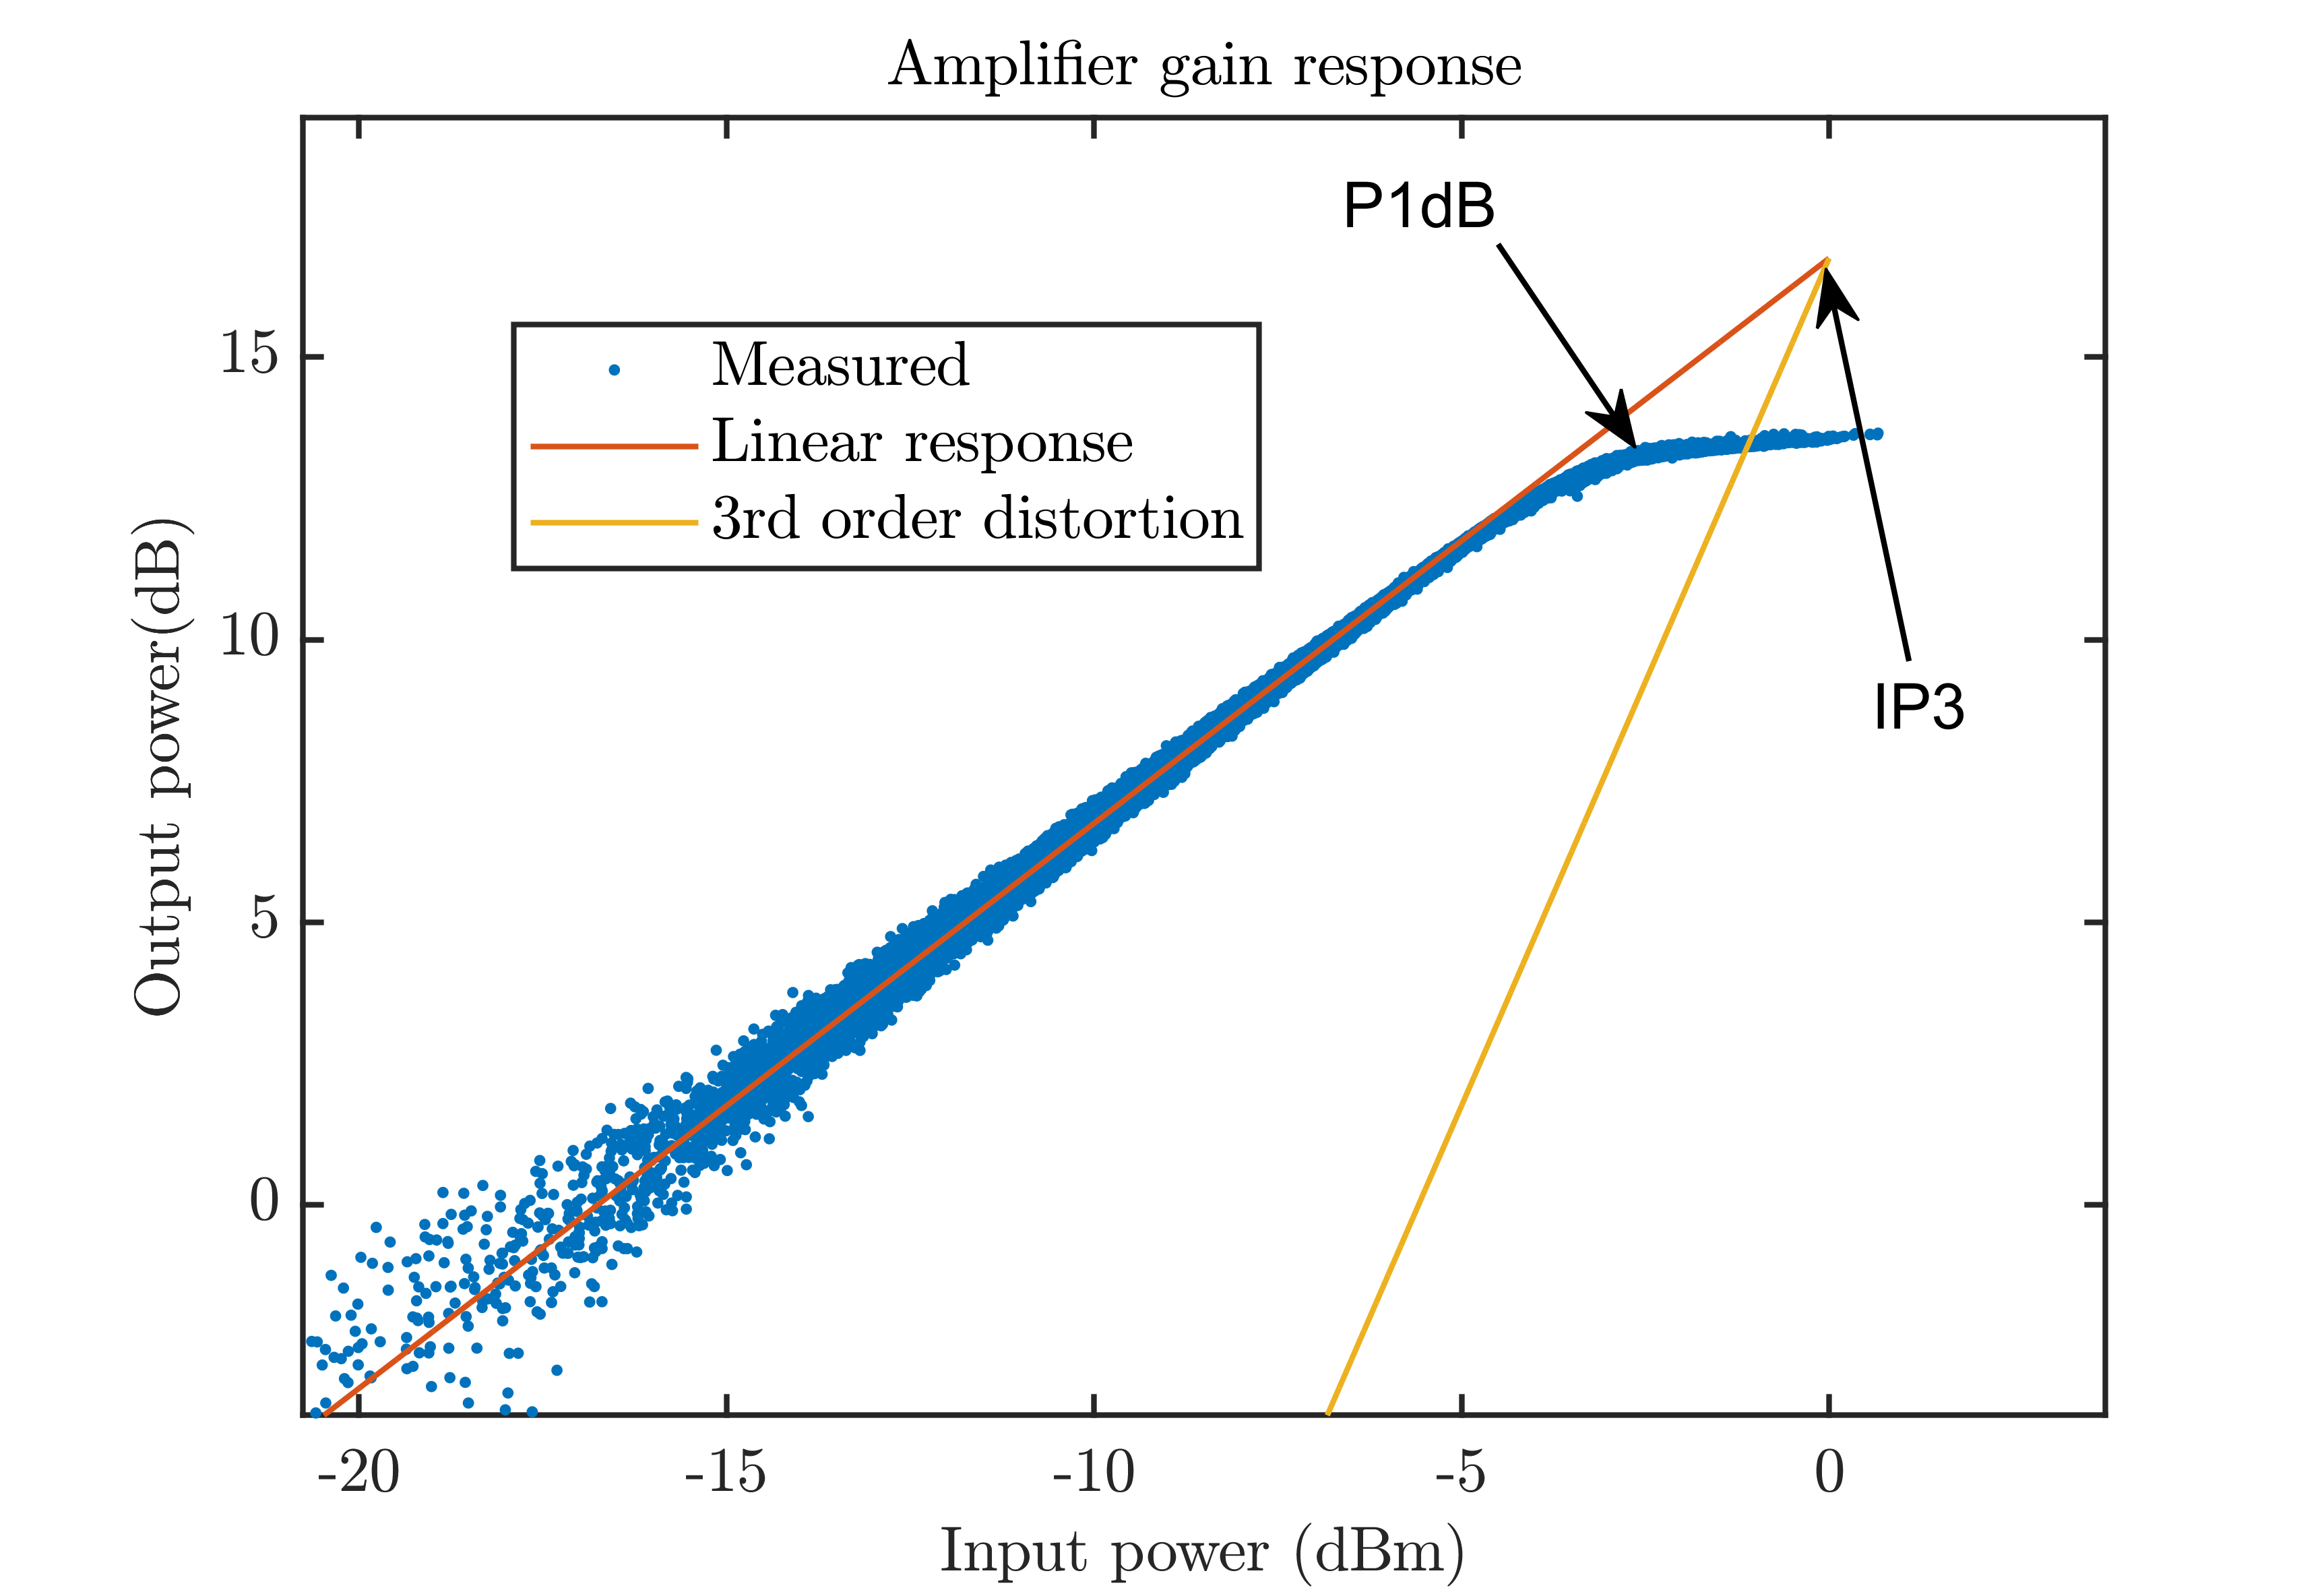
\includegraphics[scale = 0.8]{figures/ch1/amp_lin.png}
\caption{Amplifier non-linearity}
\label{fig:amp_lin}
\end{figure} 

An ideal power amplifier has an linear response over all frequencies and input power. This is depicted in \ref{fig:amp_lin} as Linear response. Unfortunately this is not true and therefore a measurement of a power amplifier has been done. The measurement shows that the amplifier at some level can be assumed linear, but at a point the amplifier will saturate due to the supply voltage and the gain will compress. The point where there is 1dB from the linear response to the real response is called the 1dB compression point (P1dB) which is also depicted in the figure. The non-linear gain response causes a distortion at the output which can be described by equation \ref{eq:dest} \citep{NI}. If a input-signal using two tones is considered then there will be a difference and a sum of the frequencies presented at the output which is caused by the cubic term in equation \ref{eq:dest2}.

\begin{equation} \label{eq:dest}
V_{out} = a_0 + a_1 V_{in} + a_2 V_{in}^2 + a_3 V_{in}^3 + a_4 V_{in}^4 + ... 
\end{equation}

Where $V_{out}$ is the output signal from the amplifier, $a_1, a_2 ,a_3..$ is coefficients describing the ratio of the distortion and $V_{in}$ is the input signal. If a single tone input is presented, then the output will consist of purely odd and even harmonic distortion. 

\begin{equation}\label{eq:dest1}
V_{in} = sin(\omega_1 t) + sin(\omega_2 t)
\end{equation} 

\begin{equation} \label{eq:dest2}
V_{out} = a_0 + a_1 (sin(\omega_1 t) + sin(\omega_2 t)) + a_2 (sin(\omega_1 t) + sin(\omega_2 t))^2 + a_3 (sin(\omega_1 t) + sin(\omega_2 t))^3 + ... 
\end{equation}

This is also called Two-Tone Third-Order Intermodulation Distortion and is also depicted in figure \ref{fig:amp_lin} as 3rd order distortion with a slope of 3:1. It can bee seen that when the output power increases then the 3rd order distortion increases 3 times. A measurement of this is called the third-order-intercept-point (IP3 or TOI). However, the intercept point it not directly measurable since the amplifier reaches compression way before. It can bee seen from figure \ref{fig:amp_psd} that the distorted component are spaced too close in frequency to be effectively filtered. This will cause distortion into nearby channels and is measured as Adjacent Chennel Power Ratio (ACPR).

\begin{figure}[H]
\centering 
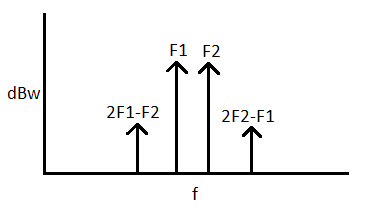
\includegraphics[scale = 0.7]{figures/ch1/amp_psd.png}
\caption{Two-Tone Third-Order Intermodulation Distortion}
\label{fig:amp_psd}
\end{figure}

%%%%%%%%%%%%%%%%%%%%%%%%%%%%%%%%%%%%%%%%%%%%%%%%%%%%%%%%%%%%%%%%%%%%%%%%%%%%%%%%%%%%%%%%%%%%%%%%%%%%%%%%%%%%%%%%%%%%
\subsubsection{Distortion due to non-linearity}

\begin{figure}[H]
\centering 
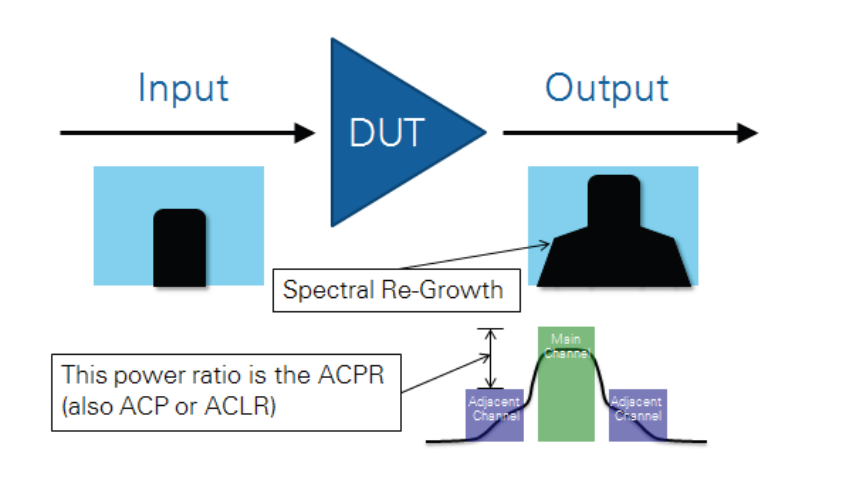
\includegraphics[scale = 0.5]{figures/ch1/acpr.png}
\caption{Graphical Depiction of ACPR in the frequency domain \citep{NI}}
\label{fig:acpr}
\end{figure}

Due to the non-linearity of the PA described before, spectral regrowth will occur which will affect nearby channels. The Adjacent Channel Power Ratio (ACPR) is a measure of the power of the distortion components, caused by the non-linearity of the PA, that are leaked into the adjacent channel see figure \ref{fig:acpr}. The formula for the ACPR is given by equation \ref{eq:acpr} and is used after a Fourier transform has been performed at the output signal of the PA.

\begin{equation} \label{eq:acpr}
	ACPR = \frac{\int_{adjch}^{} |Y(f)|^2 df }{\int_{mainch}^{} |Y(f)|^2 df}
\end{equation}   

Where $Y(f)$ is the Fourier transform of the signal, adjch is the adjacent-channel and mainch is the main-channel. 

\begin{figure}[H]
\centering 
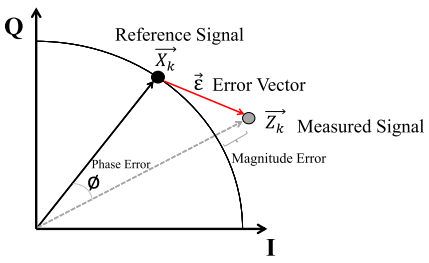
\includegraphics[scale = 0.8]{figures/ch1/evm.png}
\caption{Graphical view of the EVM}
\label{fig:evm}
\end{figure}
  
Another measure of the error is the Error Vector Measurement (EVM) or  Relative Constellation Error (RCE) which both is a measure of the error due to the constellations points in a IQ plot. If a signal is sent through an amplifier with a given IQ value, then the amplifier will distort those IQ values. The EVM and RCE is a measure of the power of the error vector divided by the power of the reference vector. \citep{ali2016}

\begin{equation} \label{eq:evm}
	EVM = \frac{P_{error}}{P_{reference}} = \frac{E[|z(t)-x(t)|^2]}{E[|x(t)^2|]}
\end{equation}  
 
\begin{figure}[H]
\centering 
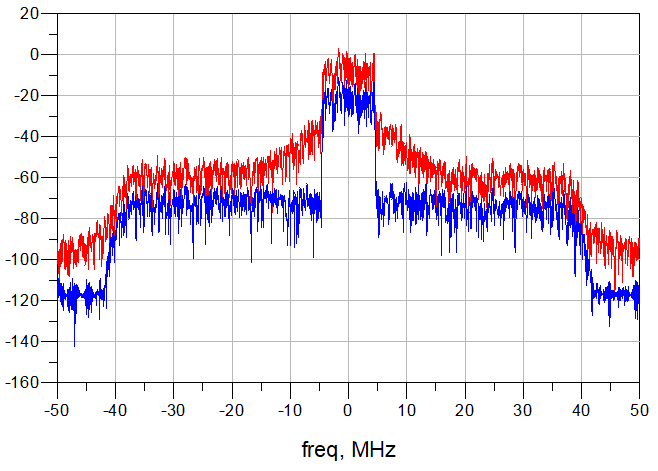
\includegraphics[scale = 0.5]{figures/ch1/ads_nonlin_dest.png}
\caption{Destortion simulated in ADS, where blue is input-signal and red is output-signal. The simulation is made with a single amplifier connected to a $50\Omega$ resistor. It is clearly that the output-signal is distorted. The ACPR becomes -45dB with a BW at 10MHZ}
\label{fig:pre_cons}
\end{figure}


\section{AM/AM and AM/PM distortion}
If the input signal to the PA is modelled as equation \ref{eq:amam1}

\begin{equation}\label{eq:amam1}
x(t) = a(t)e^{j\phi(t)}
\end{equation}

Where $a(t)$ is the envelope of the signal and $e^{j\phi(t)}$ is the phase of the input signal. Then the distorted output of the amplifier will be that of equation \ref{eq:amam1} where $g(t)$ is the amplitude distortion and $f(t)$ is the phase distortion also called Amplitude to Amplitude (AM/AM) and Amplitude to Phase (AM/PM) distortion. AM/AM distortion can be defined as the deviation from the constant gain when PA is
operated in compression region. On the other hand, the increased phase change at compression
region can be termed as AM/PM distortion.In presence of wideband signals having non constant amplitude, PA behaves as nonlinear system and exhibits two types of non-linearities which is static distortion and memory effects.  

\begin{equation}\label{eq:amam2}
y(t) = g(a(t))e^{j\phi(t)+f(a(t))}
\end{equation}

\subsubsection{Memory effects}

\begin{figure}[H]
\centering 
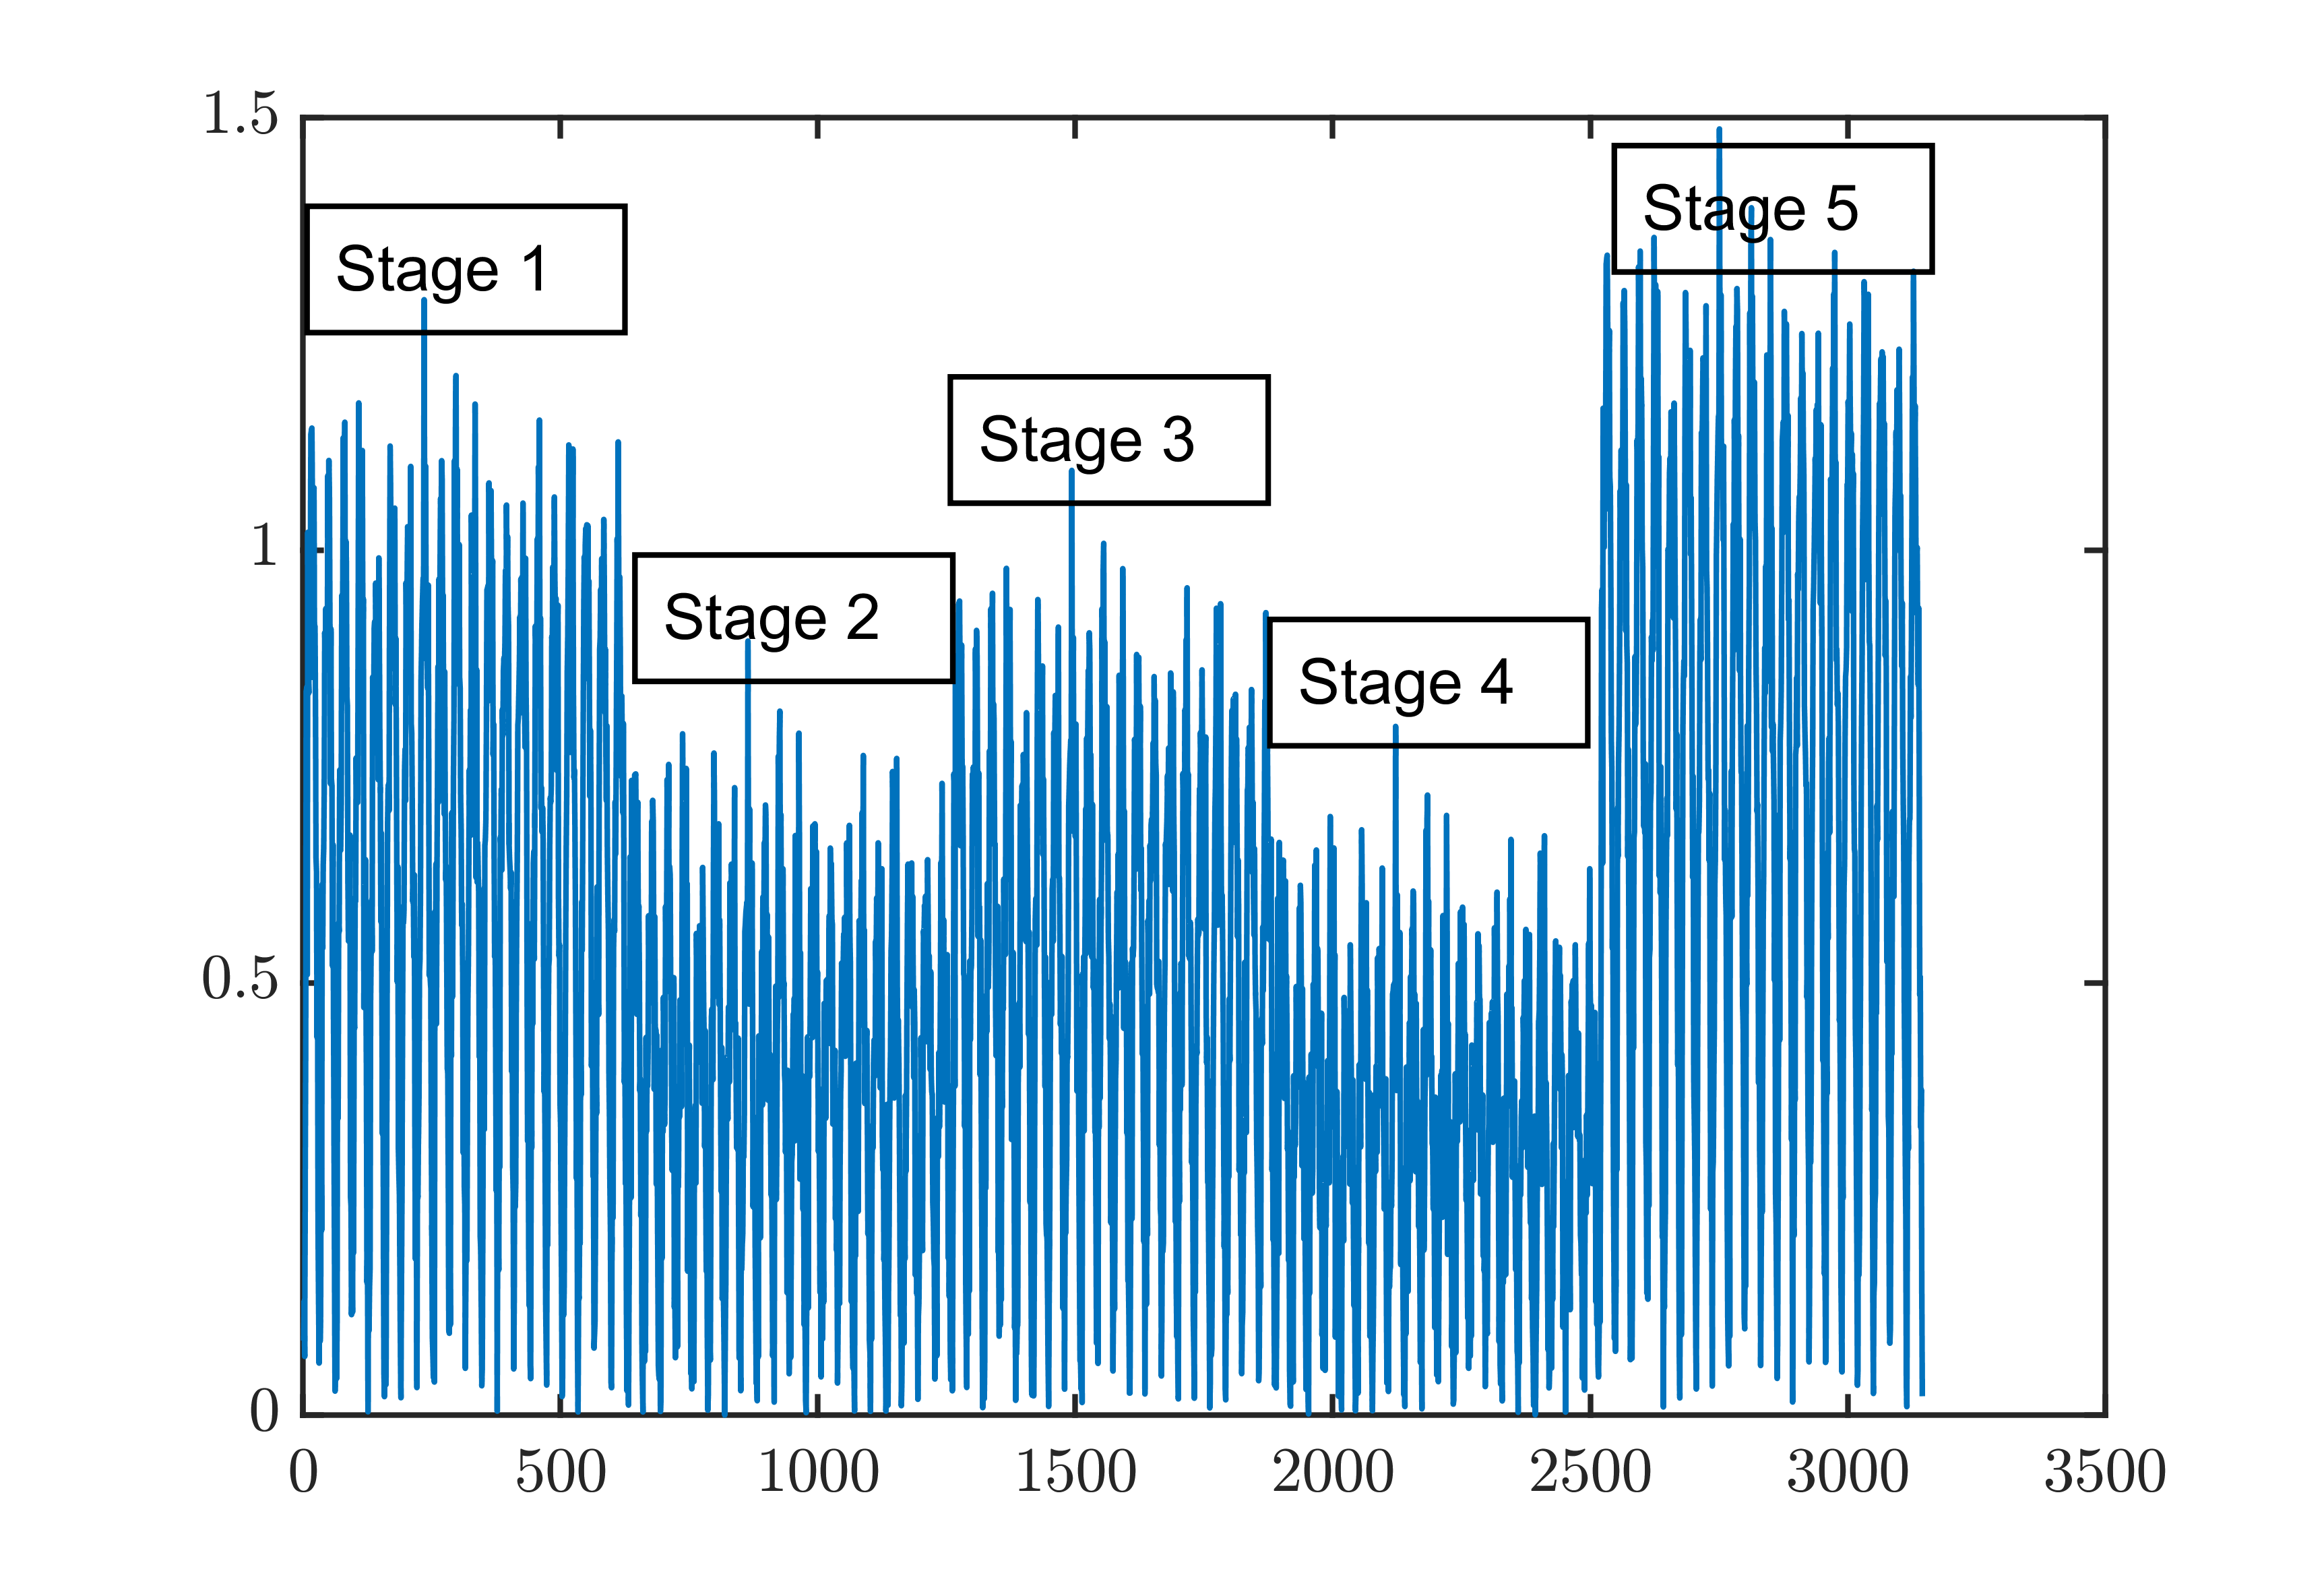
\includegraphics[scale = 0.7]{figures/ch1/amplitude.png}
\caption{Example of amplitude changes at the input of a PA }
\label{fig:mem_amp}
\end{figure}


In modern communication systems, the input power to the PA may be adjusted corresponding to the needs by the network. This makes a suddenly increase or decrease in the power as depicted in figure \ref{fig:mem_amp} which makes the PA work in the transient stage \citep{guo2015} \citep{liu2007}. The transient stage is where the power suddenly increases or decreases to another mean power, whereas the steady state is when the PA operates under stable conditions where the mean power is constant. When the PA is operated in steady state under a high mean power, the amplifier will begin to dissipate heat. This will cause the internal transistors to operate under a hot state where the characteristic of the transistors will change due to a colder state. If the mean power suddenly is decreased the amplifier will still be hot, but with time the amplifier will cool down and the characteristic will change. This can be called slow memory effects whereas fast memory effects is when the amplifier is driven in its steady state and the parasitics of the components distort the signal. Also antennas at the output of the amplifier has an important role specially if several antennas are connected to form an array. The electrical field will couple to each other and cause fields that will affect the memory effects in the system. 


\section{Efficiency}
An important measure of an amplifier is its efficiency, specially when the amplifier is located in a battery powered application. The efficiency of a amplifier is given by equation \ref{eq:effi}

\begin{equation} \label{eq:effi}
\eta = \frac{P_{out}}{P_{amplifier}+P_{out}} = \frac{P_{out}}{P_{DC}}
\end{equation}

Where $P_{out}$ is output power from the amplifier, $P_{amplifier}$ is power dissipated in the amplifier and $P_{DC}$ is the power DC consumption. A more common way to express the efficiency is in terms of power added efficiency (PAE) which is a measure of the difference of power between the output and the input signals versus the DC power consumption.

\begin{equation} \label{eq:effi2}
PAE = \frac{P_{out}-P_{in}}{P_{DC}}
\end{equation}
 


%%%%%%%%%%%%%%%%%%%%%%%%%%%%%%%%%%%%%%%%%%%%%%%%%%%%%%%%%%%%%%%%%%%%%%%%%%%%%%%%%%%%%%%%%%%%%%%%%%%%%%%%%%%%%%%%%%%%
\section{Antenna Diversity and MIMO}

\begin{figure}[H]
\centering 
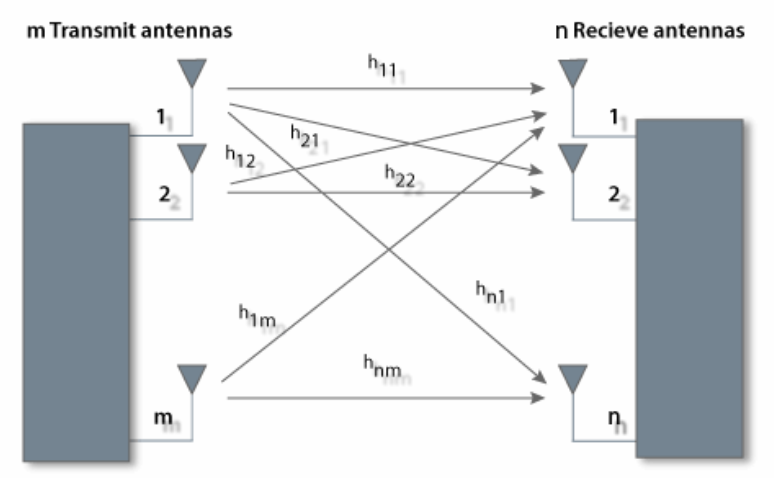
\includegraphics[scale = 0.4]{figures/ch1/mimo.png}
\caption{Concept of MIMO \citep{silvus2019}}
\label{fig:mimo}
\end{figure}

MIMO (Multiple Input Multiple Output) systems are systems with Multiple Element Antennas at both link ends. The antenna elements of a MIMO system can be used for four different purposes: beamforming, diversity, interference suppression, and spatial multiplexing which is transmission of several data streams in parallel that allows improvement of capacity.\citep{molisch2011} A MIMO system is modelled as in equation \ref{eq:mimo} and is also depicted in figure \ref{fig:mimo}.

\begin{equation}\label{eq:mimo}
\textbf{y = Hx+n}
\end{equation}  

Where \textbf{y} is the received vector, \textbf{H} is the channel matrix, \textbf{x} is the transmitted vector and \textbf{n} is noise. The principle of MIMO is to ensure that the same information reaches the receiver on several
statistically independent channels. In MIMO systems, several transmits paths is archived by use of several antennas, which gives a spatial separation if they are separated enough to give a correlation factor $\rho$ that is below $0.5 - 0.7$ \citep{molisch2011}. The formula for the envelope correlation factor between two antennas is given by equation \ref{eq:corr_fac}. The formula assumes that the WSSUS (Wide-Sense Stationary Uncorrelated Scattering) model is valid, no LOS exists, the power delay profile has an exponential shape, the incident power is isotropically distributed in azimuth and only propagates in the horizontal plane, and an omnidirectional antenna is used.

\begin{eqnarray} \label{eq:corr_fac}
\rho = \frac{J_0^2( k_0 v \tau)}{1+(2\pi)^2 S_\tau^2(f_2 - f_1)^2 }
\end{eqnarray}      

Where $J_0$ is the Bessel function of the first kind and $S_\tau$ is the delay-spread of the channels. If the correlation between two antennas is investigated for the same frequency, then the formula can be rewritten as equation \ref{eq:corr_fac_re} because $f2-f1=0$.

\begin{eqnarray} \label{eq:corr_fac_re}
\rho = J_0^2( 2\pi d)^{-1}
\end{eqnarray} 

Where $d$ is the element spacing given in wavelengths. A plot of this can bee seen in figure \ref{fig:correlation}.

\begin{figure}[H]
\centering 
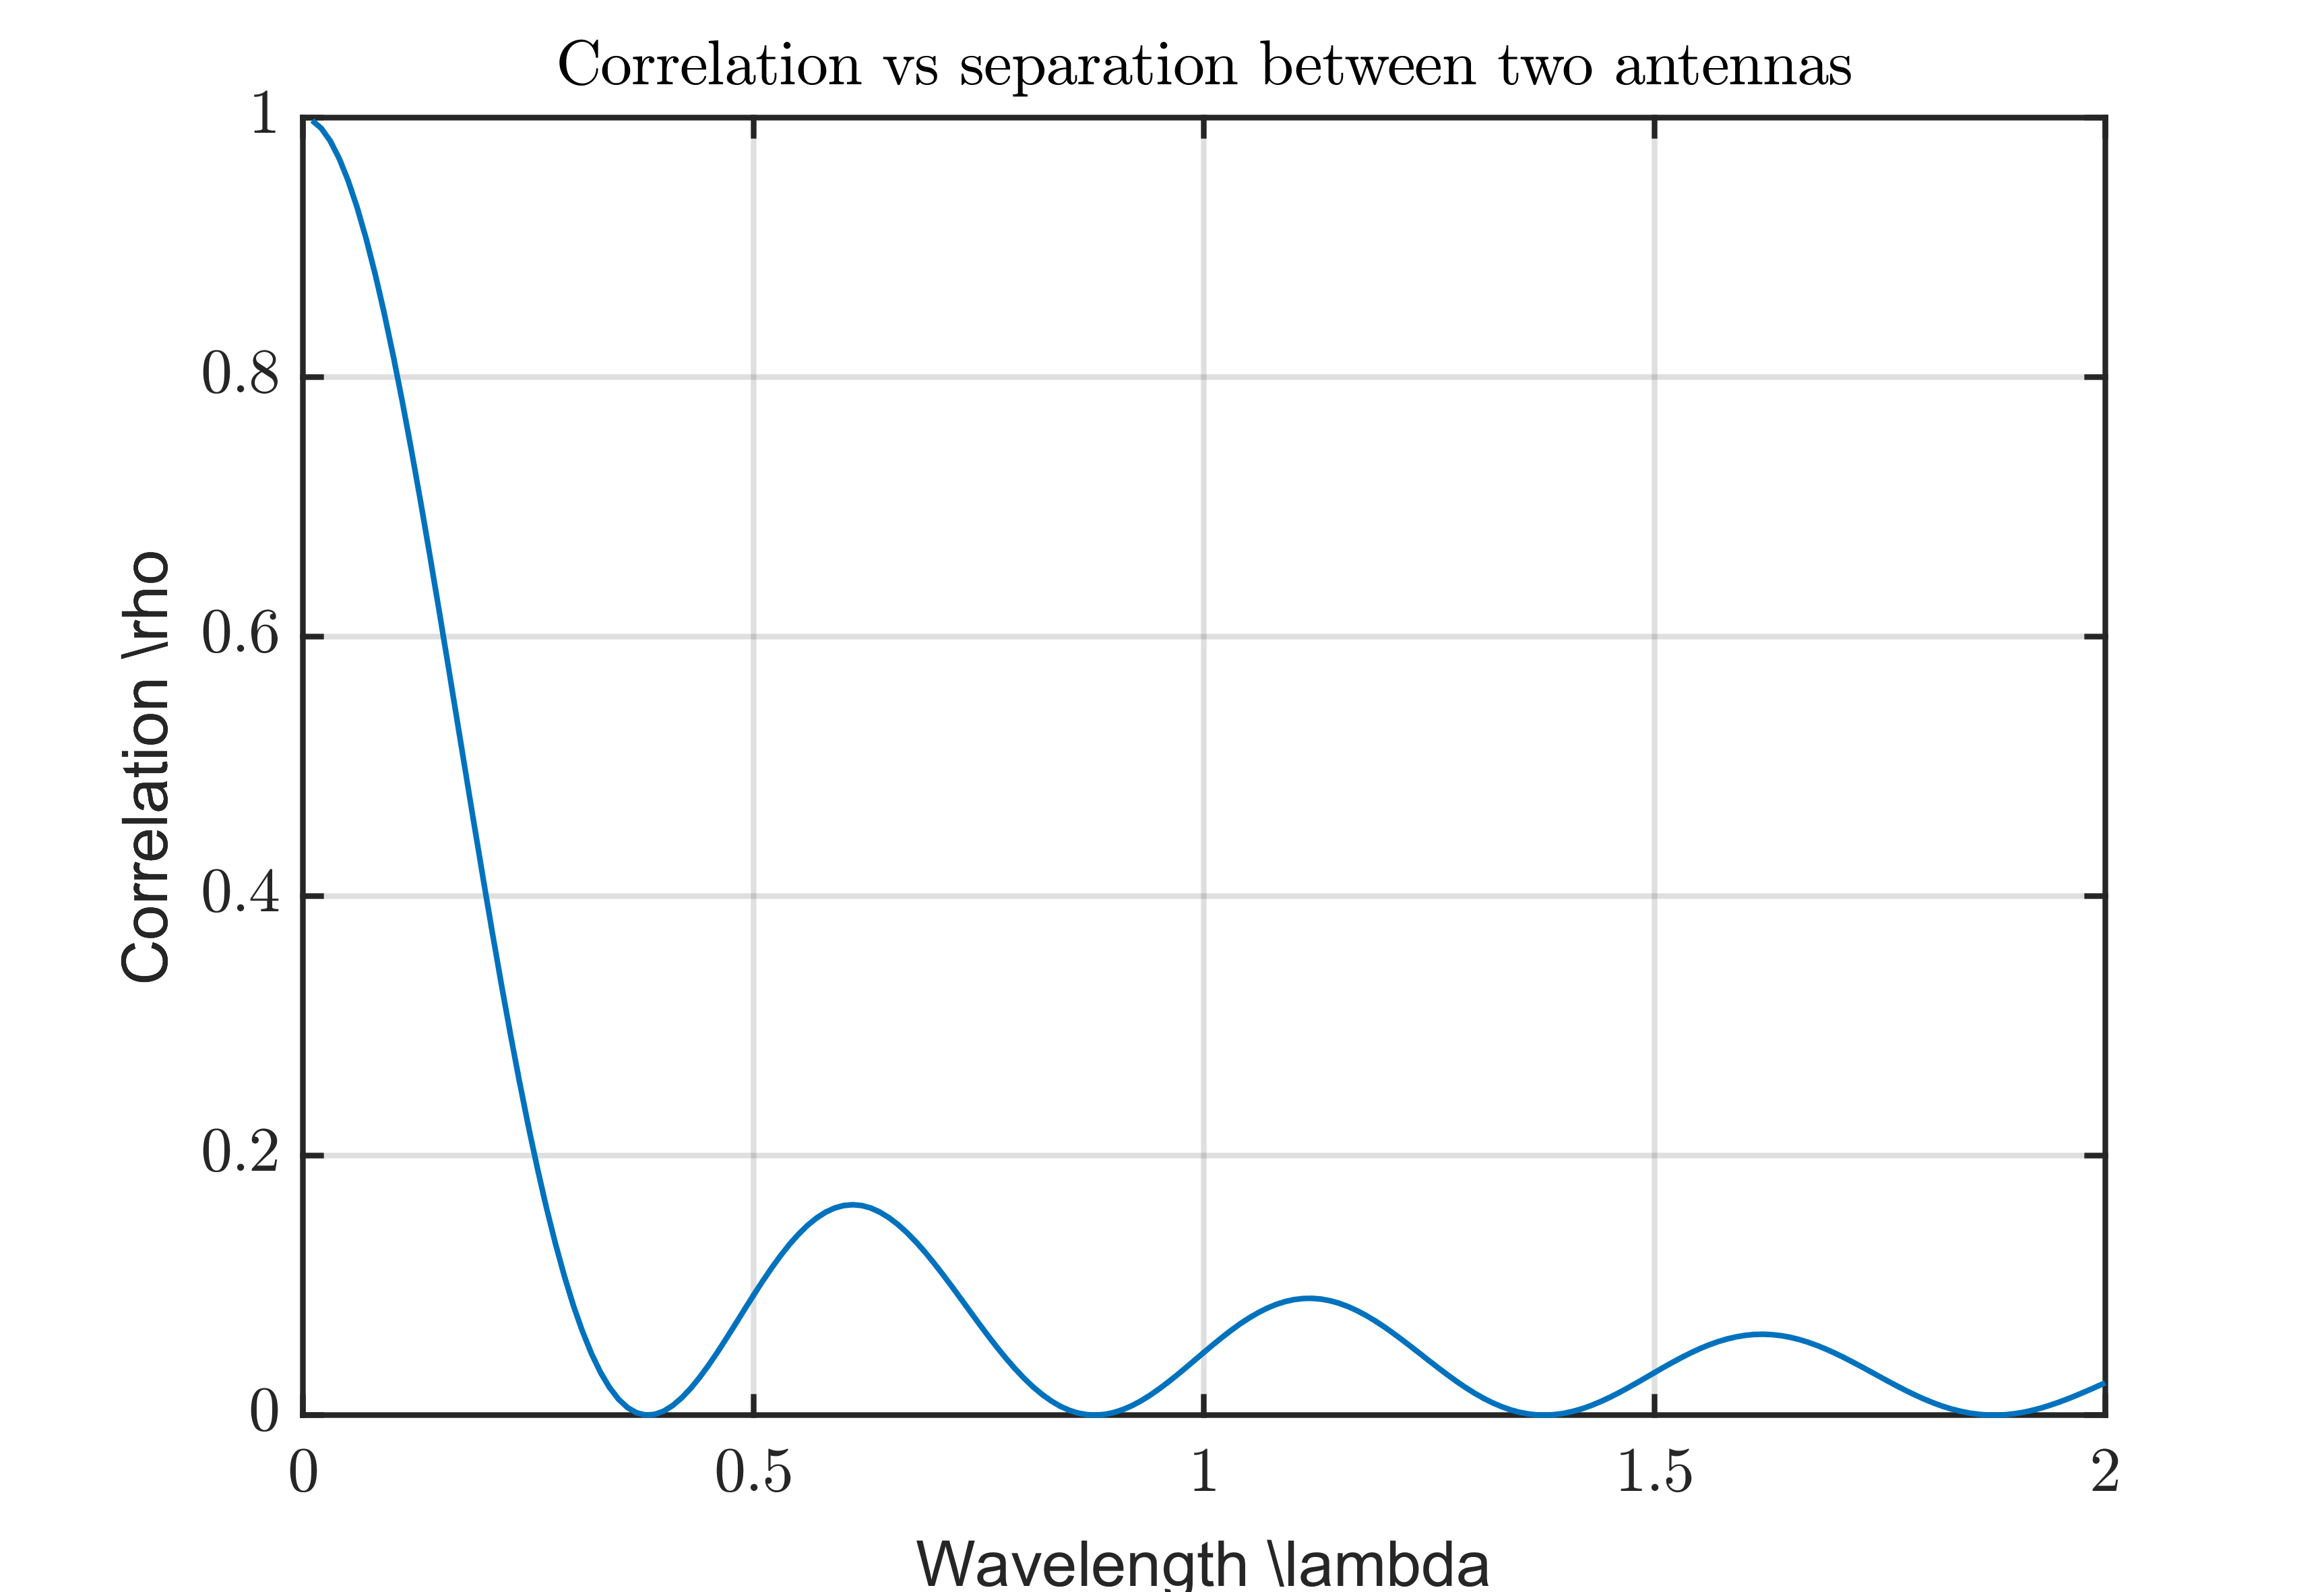
\includegraphics[scale = 0.7]{figures/ch1/correlation.png}
\caption{Correlation factor for two antennas versus distance}
\label{fig:correlation}
\end{figure}

Another method to calculate the correlation factor is to use measured or simulated S-parameters as shown in equation \ref{eq:spar_corr} \citep{wang2011} where k is the propagation constant and d the distance in meters. 

\begin{equation} \label{eq:spar_corr}
\rho = \frac{A+B J_0(kd)}{B+A J_0(kd)}
\end{equation}

\begin{equation} 
A = -2Re(S_{12}^*(1-S_{11}))
\end{equation}

\begin{equation} 
B = |1-S_{11}|^2 + |S_{12}|^2
\end{equation}


%%%%%%%%%%%%%%%%%%%%%%%%%%%%%%%%%%%%%%%%%%%%%%%%%%%%%%%%%%%%%%%%%%%%%%%%%%%%%%%%%%%%%%%%%%%%%%%%%%%%%%%%%%%%%%%%%%%

\section{Array factor}
When several antennas are spaced relatively close to each other it is called an antenna array. If the antennas are isotopic and are spaced with a quarter wavelength then the array will radiate twice the energy in the direction perpendicular to the array, thou the gain along the array will become zero. A mathematical expression of this is called the array factor (AF).

\begin{equation}
AF = \sum_{n=1}^{N} e^{(n J 2\pi d \cos(\alpha)+JB(n))}
\end{equation}

Where N is number of antennas in the array, d is the distance between the antennas, $\alpha$ is the azimuth angle from $0..2\pi$ and B is the feeding phase of a single antenna. In figure \ref{fig:af_2ant} and \ref{fig:af_4ant} the array factor for 2 and 4 antennas spaced $[0.1, 0.2, 0.3, 0.4, 0.5, 0.6]\lambda$ are plotted respectively. It is seen that the energy doubles in the $90^\circ$ for all distances in figure \ref{fig:af_2ant} while it becomes 4 times greater in figure \ref{fig:af_4ant}.   


\begin{figure}[H]
\centering 
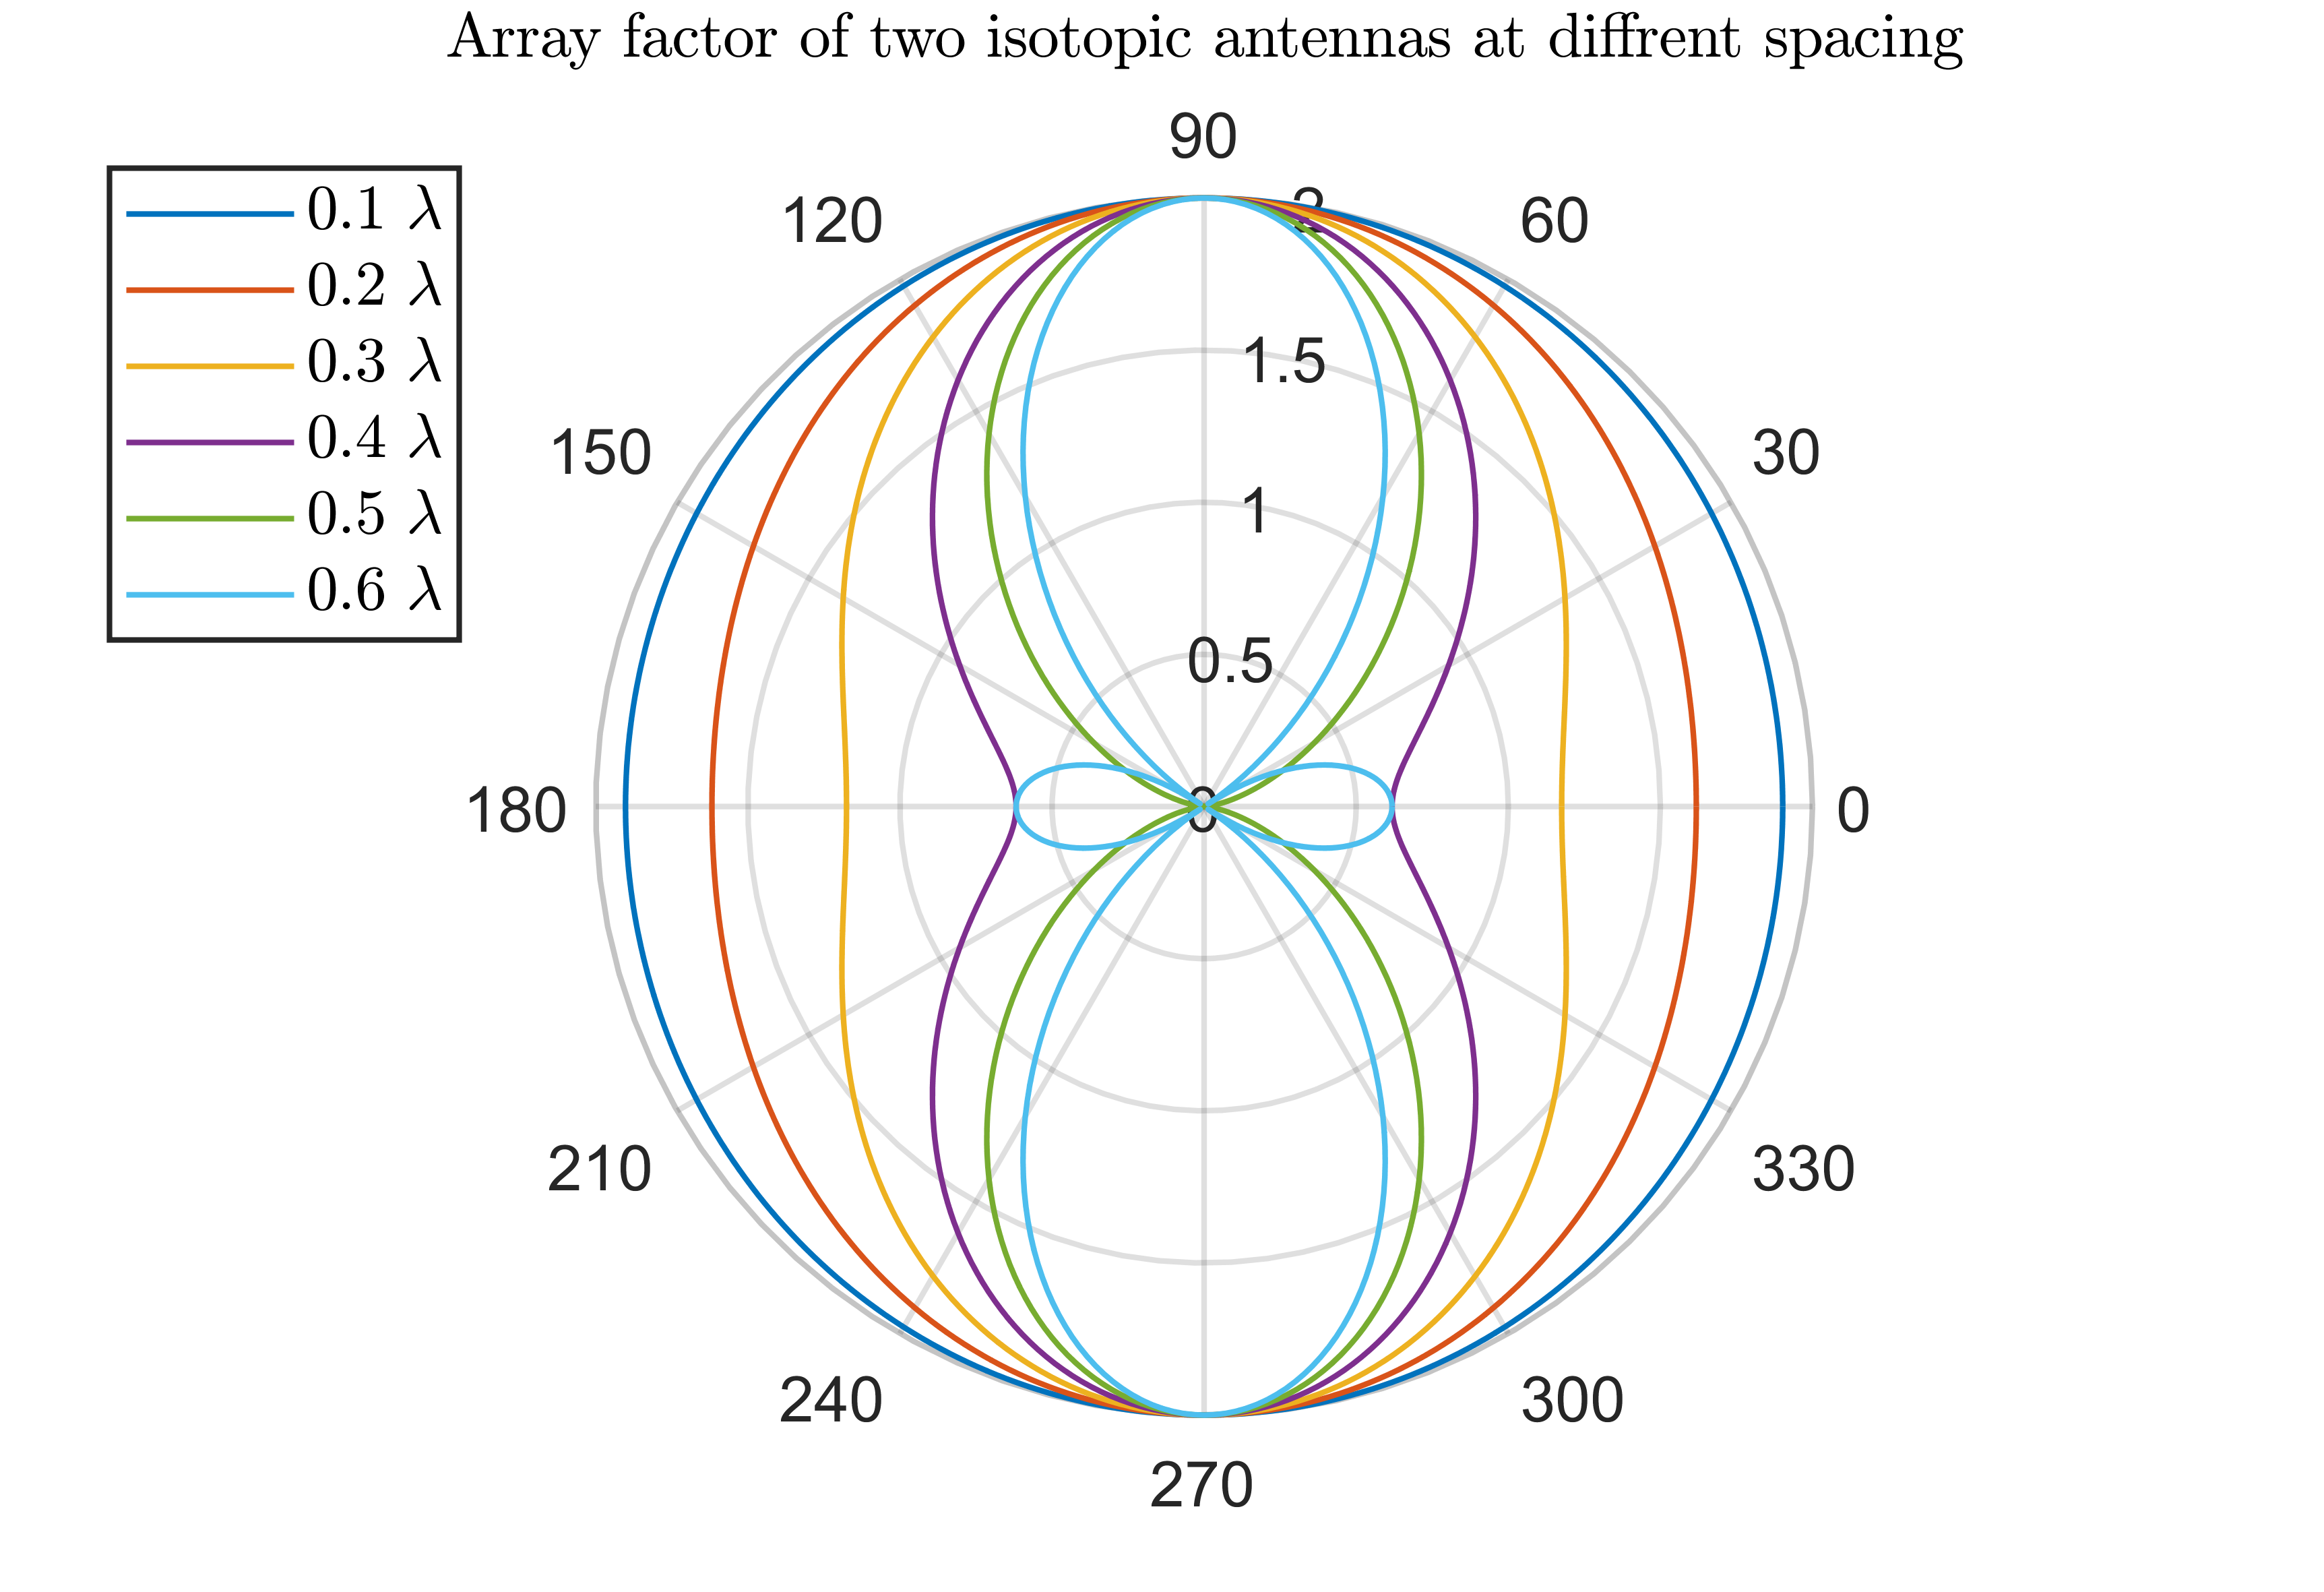
\includegraphics[scale = 0.7]{figures/measurement/af_2ant.png}
\caption{Array factor of two antennas with diffrent spacing}
\label{fig:af_2ant}
\end{figure}


\begin{figure}[H]
\centering 
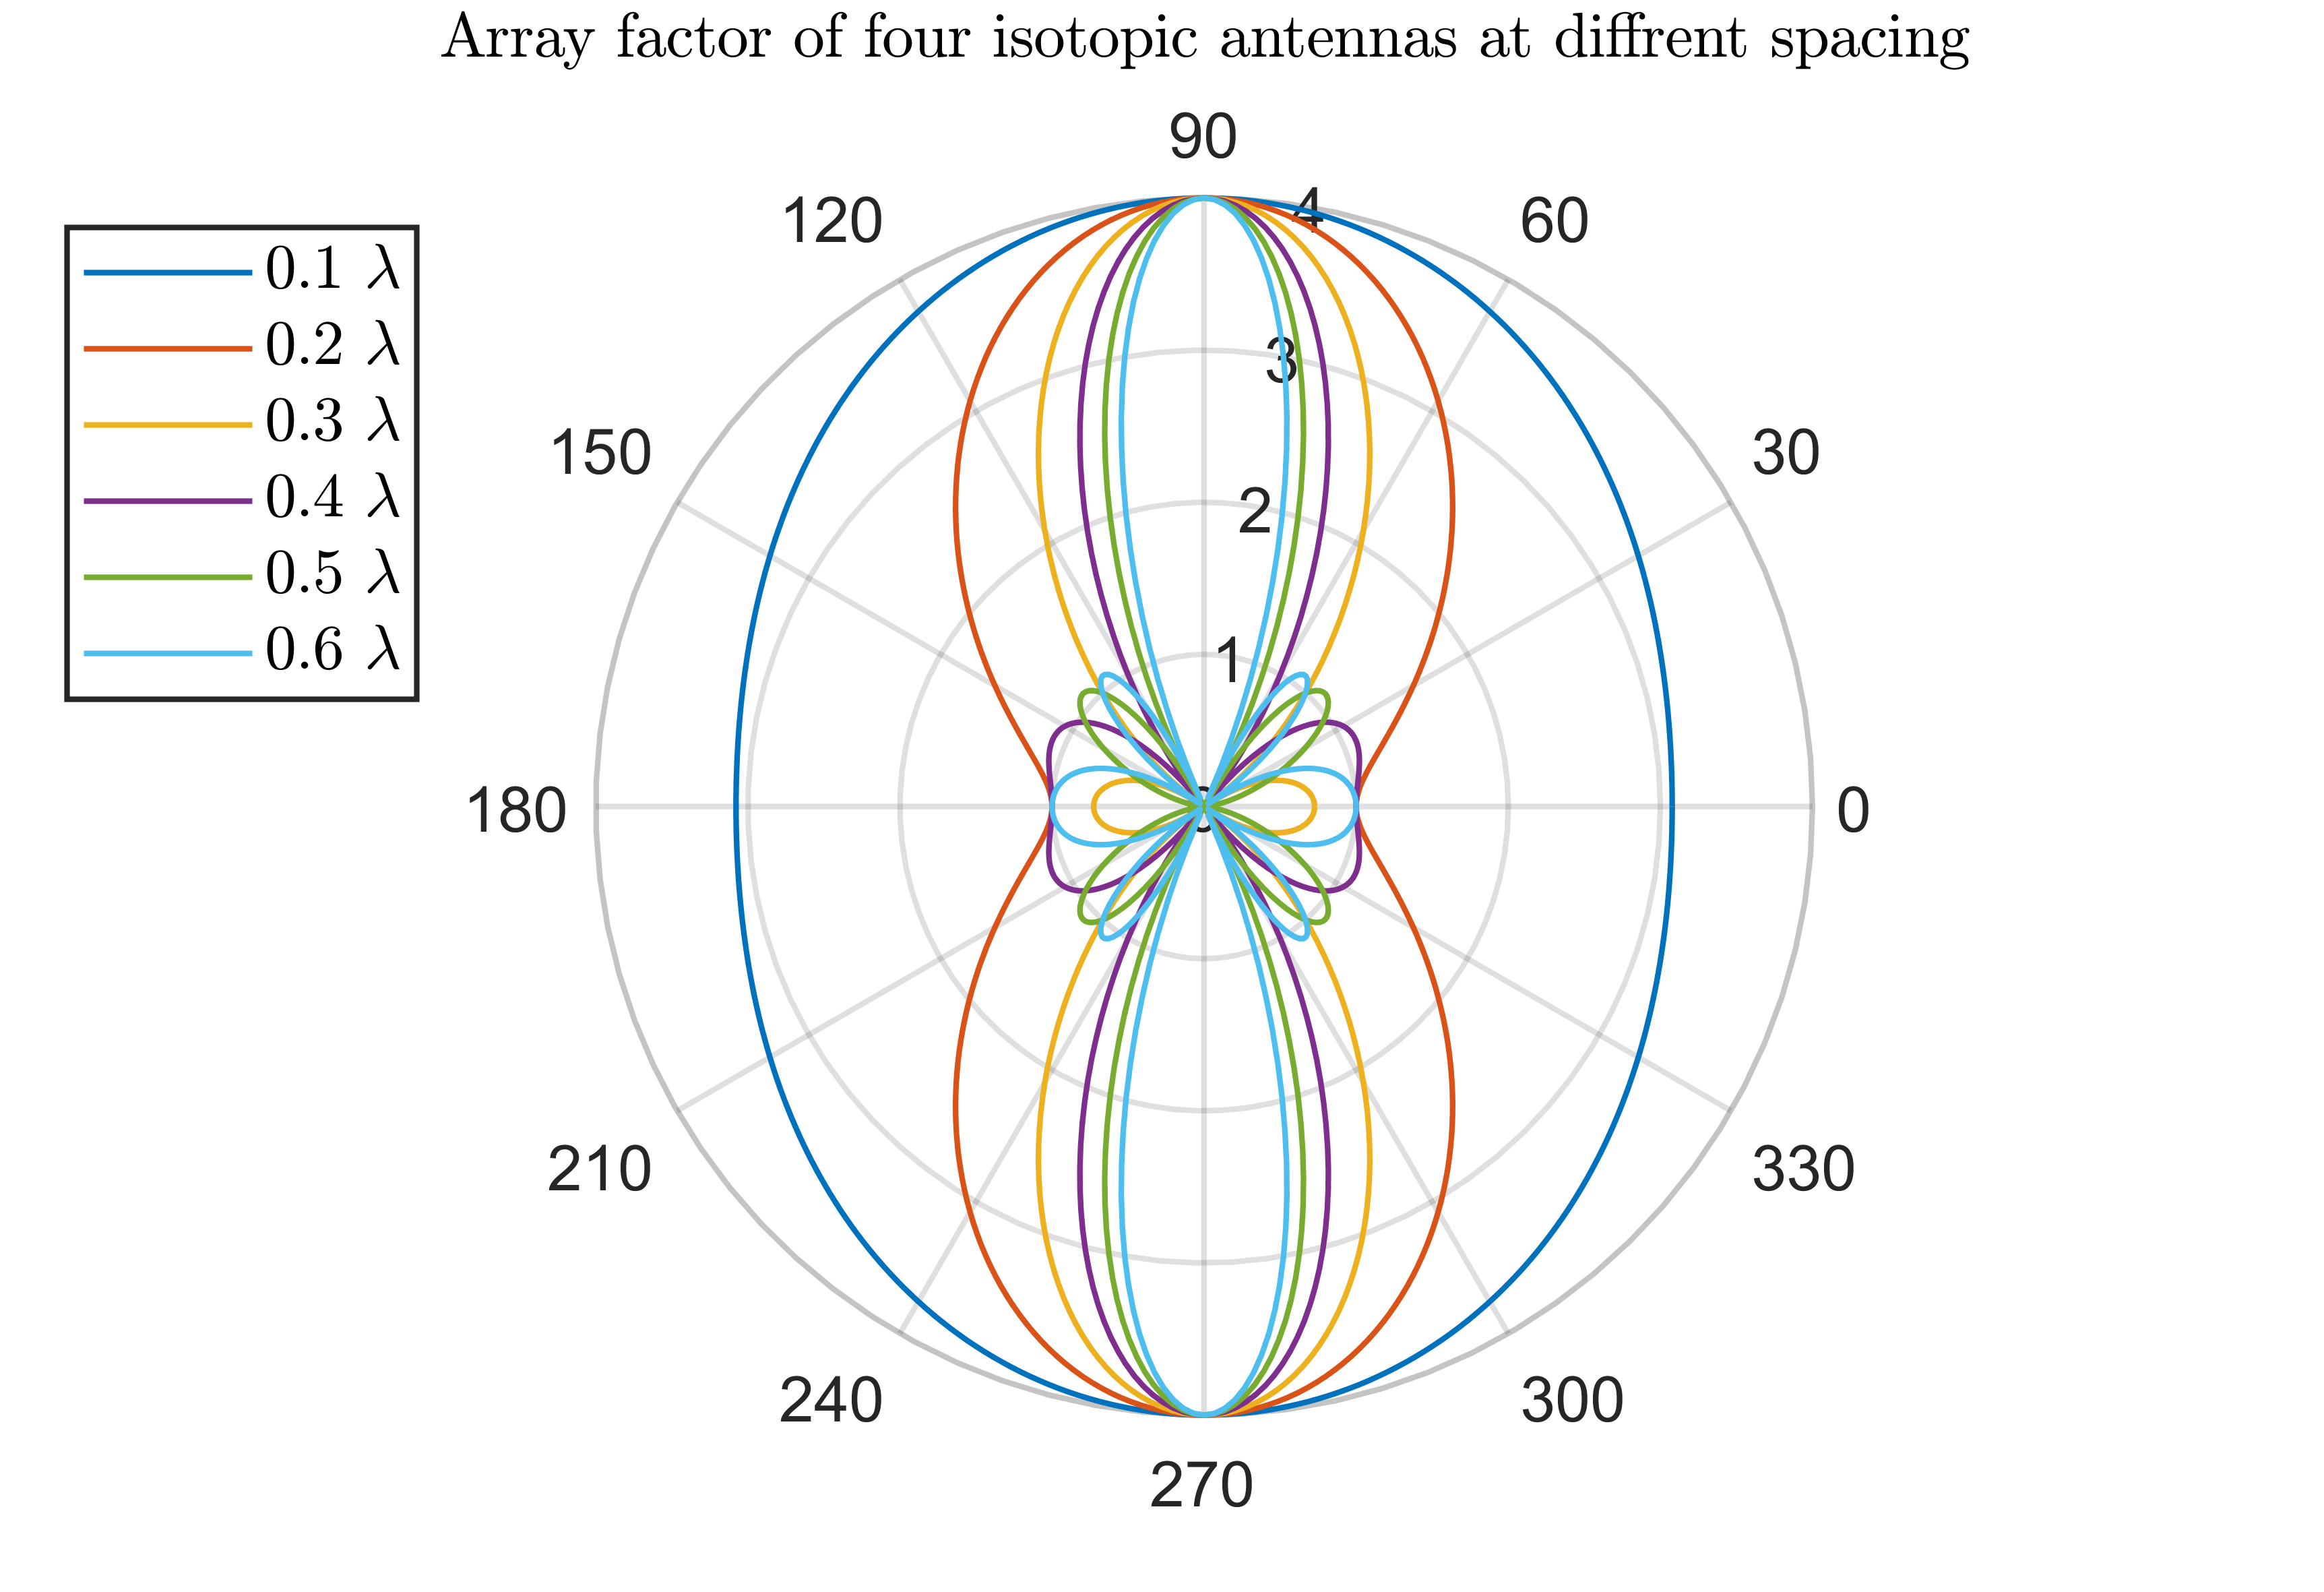
\includegraphics[scale = 0.7]{figures/measurement/af_4ant.png}
\caption{Array factor of four antennas with diffrent spacing}
\label{fig:af_4ant}
\end{figure}






